\documentclass[../../main.tex]{subfiles}
\begin{document}
\chapter{Facial Expressions}
\label{ch:facial_expressions}

Facial expressions are a crucial element of communication in both spoken and sign languages. In sign languages, they serve a dual purpose: conveying the emotional state of the signer and encoding grammatical information such as questions, negation, and emphasis. While spoken languages rely on tone and intonation for these functions, sign languages depend heavily on non-manual signals, particularly facial expressions, to fully convey the meaning of an utterance. Therefore, creating accurate and expressive facial animations in signing avatars is essential for producing realistic and comprehensible sign language content.

However, synthesizing facial expressions for signing avatars presents significant challenges due to the complexity and subtlety of these expressions. Unlike manual signs, which involve distinct hand and arm movements, facial expressions require the coordinated movement of various facial muscles, each contributing to the overall expression. Different facial features, such as eyebrows, eyes, and mouth, often move independently yet in harmony to produce coherent expressions. Moreover, the same facial expression can convey different meanings depending on the context, adding another layer of complexity to the task.

This chapter tackles these challenges by introducing a method for synthesizing facial expressions using the AZee framework for French Sign Language (LSF). To achieve this, specific production rules for facial expressions were integrated into AZee. By employing action units (AUs) as the foundational elements of these expressions, we can generate blendshapes that precisely represent the required facial movements. These blendshapes are subsequently integrated into a facial rigging system, allowing for the dynamic and realistic animation of signing avatars.

Previous chapters focused on the synthesis of manual features in sign language. In contrast, this chapter centers on the synthesis of facial expressions using the AZee framework, emphasizing their critical role in both emotional communication and the conveyance of grammatical information in sign languages. The precise synthesis of these expressions is therefore essential for enhancing the realism and effectiveness of signing avatars.

The chapter is structured as follows: Section \ref{ch:facial_expressions:related_work} reviews related work in facial expression synthesis, examining previous approaches, the challenges encountered, and recent advancements. Section \ref{ch:facial_expressions:related_work:facial_expressions_in_sign_language_synthesis} focuses on the synthesis of facial expressions in sign language avatars, discussing their importance for sign language comprehension and the challenges in capturing their nuances. Section \ref{ch:facial_expressions:related_work:face_rigging} explores different face rigging techniques, including blendshape-based rigging, skeleton-based rigging, and hybrid methods, and compares their advantages and disadvantages. Finally, Section \ref{ch:facial_expressions:related_work:emotion_recognition} delves into emotion recognition systems and their role in generating facial expressions that align with the emotional tone of the signed message.

\section{Related Work}
\label{ch:facial_expressions:related_work}

This section reviews the previous work in facial expression synthesis, focusing on the challenges and advancements in capturing the nuances of facial movements. It also discusses the importance of facial expressions in sign language synthesis and the techniques used to model these expressions effectively.

\subsubsection{Facial Expressions Synthesis}
\label{ch:facial_expressions:related_work:facial_expressions_synthesis}

todo citations
Most of the facial expressions research is motivated by synthesis from voice signals. These methods are generally categorized into lip-sync techniques [19, 39, 5, 33], which align mouth movements with audio, and full-face expression synthesis [9, 14, 53]. Some approaches model speaking style with 3D animation parameters [7], create generalized latent audio expressions combined with a person-specific 3D model [42], and produce expressive facial outputs conditioned on style, although some are unsuitable for tasks requiring full-face movement [46]. A related work, MakeItTalk [54], introduces a two-stage deep learning model that predicts facial landmark displacements based on audio input and a speaker identifier, followed by an image-to-image translation method to generate the final facial expression. Another study, EAMM [20], focuses on transferring local emotional deformations to an audio-driven talking face, using deep learning to map audio to keypoints and their dynamics, resulting in emotion-related facial motions.

Synthesis of facial expressions in sign language is a much-less explored area. SGNify \cite{Forte_2023_CVPR} can do a 3D reconstruction of a signer's face using in FLAME \cite{todo_flame} space from a monocular video. The Paula avatar uses rotational pivots and pre-defined movements, offering more natural and expressive facial animations \cite{johnson-2022-improved}. More recent work \cite{azevedo2024empowering} uses sentiment and semantic information to generate realistic facial expressions, achieving state-of-the-art results and outperforming existing approaches. However, these methods are limited in their ability to capture the full range of facial expressions in sign language, particularly the grammatical and emotional nuances that are essential for effective communication. However, these methods are limited in their ability to meaningully relate facial expressions to the signed message.

\subsection{Emotion Recognition}
\label{ch:facial_expressions:related_work:emotion_recognition}

Emotion recognition systems typically use machine learning algorithms to analyze facial features and identify the underlying emotional state. These systems can be trained on large datasets of facial images, which are annotated with emotional labels, to learn the relationships between facial movements and emotions. The most common approach to define emotions is the Ekman's Facial Action Coding System (FACS) \cite{ekman1978facial}, which categorizes facial expressions into a set of action units (AUs) (figure \ref{fig:action_units})  that correspond to specific muscle movements. Recent works by \cite{luo2022learning} have shown that deep learning models can infer the set of active action units on a face image, which can be used to predict the underlying emotion. EMOCA \cite{danvevcek2022emoca} is another work which reconstructs 3D faces from single images, accurately capturing emotional expressions by introducing an emotion-consistency loss, significantly improving the quality of reconstructed expressions over previous methods.

\begin{figure}
    \centering
    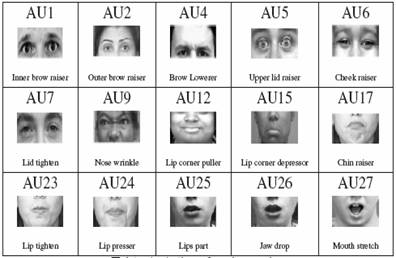
\includegraphics[width=0.8\textwidth]{chapters/facial_expressions/images/action_units.png}
    \caption{Facial Action Coding System (FACS) action units}
    \label{fig:action_units}
\end{figure}

Emotion recognition can be helpful in understanding as well as modeling facial expressions in sign language synthesis. By analyzing the emotional content of a signed message, we can generate facial expressions that align with the emotional tone of the message, enhancing the realism and expressiveness of the signing avatar.

\subsection{Face Rigging}
\label{ch:facial_expressions:related_work:face_rigging}

Face rigging is the process of creating a digital framework that allows for the animation of facial expressions. There are several approaches to face rigging, each with its advantages and disadvantages. The most common approaches include blendshape-based rigging and skeleton-based rigging.

\subsubsection{Blendshape-Based Rigging}
\label{ch:facial_expressions:related_work:face_rigging:blendshape_based_rigging}

Blendshape-based rigging involves creating a set of predefined facial shapes (blendshapes) that represent various expressions. These blendshapes can be blended together in different proportions to create a wide range of facial expressions. This method is widely used in the animation industry due to its simplicity and flexibility. It allows animators to create complex expressions by adjusting the influence of each blendshape on the final animation. However, the downside of this approach is that it requires a large number of blendshapes to capture all possible expressions, which can be time-consuming to create and manage.

Blendshapes are particularly effective for capturing specific facial movements, such as eyebrow raises, lip curls, cheek puffs, etc. By creating a library of blendshapes that correspond to different facial actions, animators can easily combine these shapes to create expressive and realistic facial animations (figure \ref{fig:blendshapes}).

\begin{figure}
    \centering
    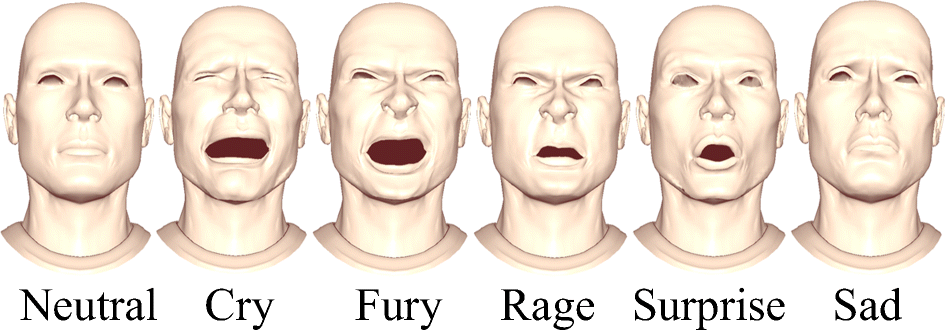
\includegraphics[width=0.8\textwidth]{chapters/facial_expressions/images/blendshapes.png}
    \caption{Blendshapes for facial expressions}
    \label{fig:blendshapes}
\end{figure}

\subsubsection{Skeleton-Based Rigging}
\label{ch:facial_expressions:related_work:face_rigging:skeleton_based_rigging}

Skeleton-based rigging, also known as joint-based rigging, uses a hierarchical system of bones and joints to control facial movements. This approach is more commonly used for animating body movements but can also be applied to facial animation. The advantage of skeleton-based rigging is that it provides a more ways to control since the control space of joints can be 3D (figure \ref{fig:skeleton_based_rigging}). Example, jaw movements(up, down, left, right, front or back), eye movements, etc. However, it can be less intuitive to work with compared to blendshapes, especially for subtle expressions that require precise control over individual facial muscles.

\begin{figure}
    \centering
    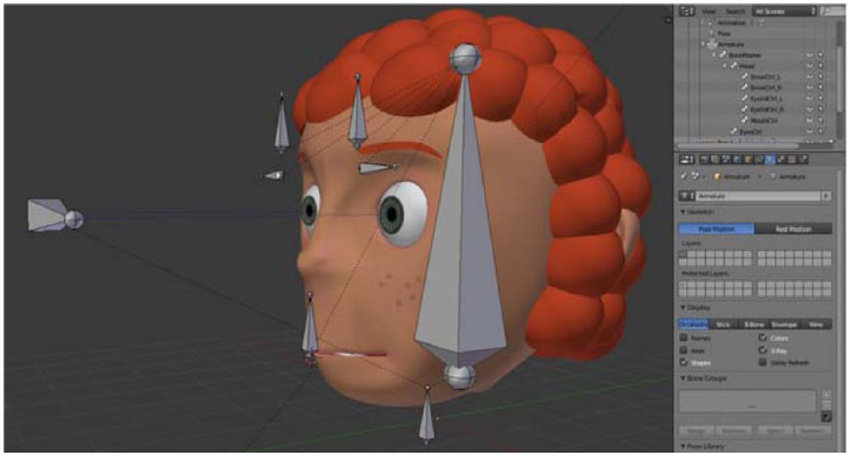
\includegraphics[width=0.8\textwidth]{chapters/facial_expressions/images/skeleton_based_rigging.png}
    \caption{Skeleton-based rigging for facial expressions}
    \label{fig:skeleton_based_rigging}
\end{figure}

\subsubsection{Hybrid Rigging}
\label{ch:facial_expressions:related_work:face_rigging:hybrid_rigging}

Hybrid rigging approaches combine elements of both blendshape-based and skeleton-based rigging to offer greater flexibility and control. By leveraging the strengths of both techniques, hybrid rigging can overcome the limitations of each individual approach. For example, blendshapes can be used for fine-tuned expressions, while skeletons provide control over broader movements like jaw or head rotations. 

\subsection{Capturing Facial Expressions}
\label{ch:facial_expressions:related_work:face_rigging:capture}

Keyframing remains a foundational technique in facial animation, where animators manually set key poses and interpolate between them to create fluid motion. While keyframing is effective in controlled environments, it may struggle to capture the natural variability and complexity required in sign language synthesis, where subtle changes in expression can convey different meanings.

\begin{figure}
    \centering
    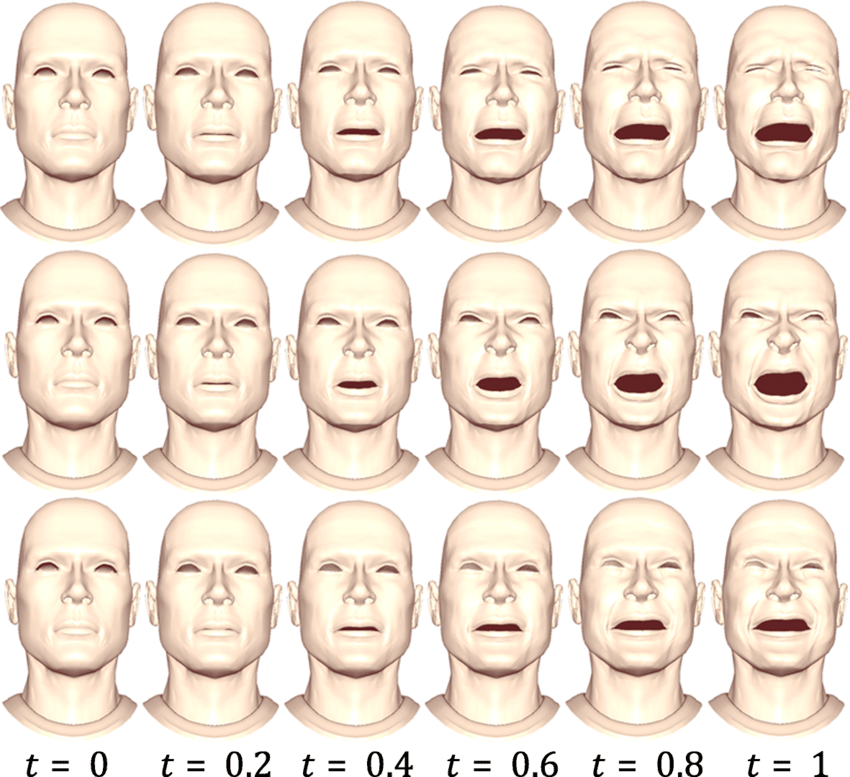
\includegraphics[width=0.8\textwidth]{chapters/facial_expressions/images/keyframing.png}
    \caption{Keyframing process, showing how key poses are set and interpolated to create a continuous animation.}
    \label{fig:keyframing}
\end{figure}

Performance-based approaches, such as motion capture, involve capturing real human facial movements and using this data to drive digital avatars. This method provides a high level of realism, capturing the natural dynamics and nuances of facial expressions. Apple's ARKit and FaceCap are examples of performance-based facial animation tools that use motion capture technology to animate digital characters (figure \ref{fig:motion_capture}).

\begin{figure}
    \centering
    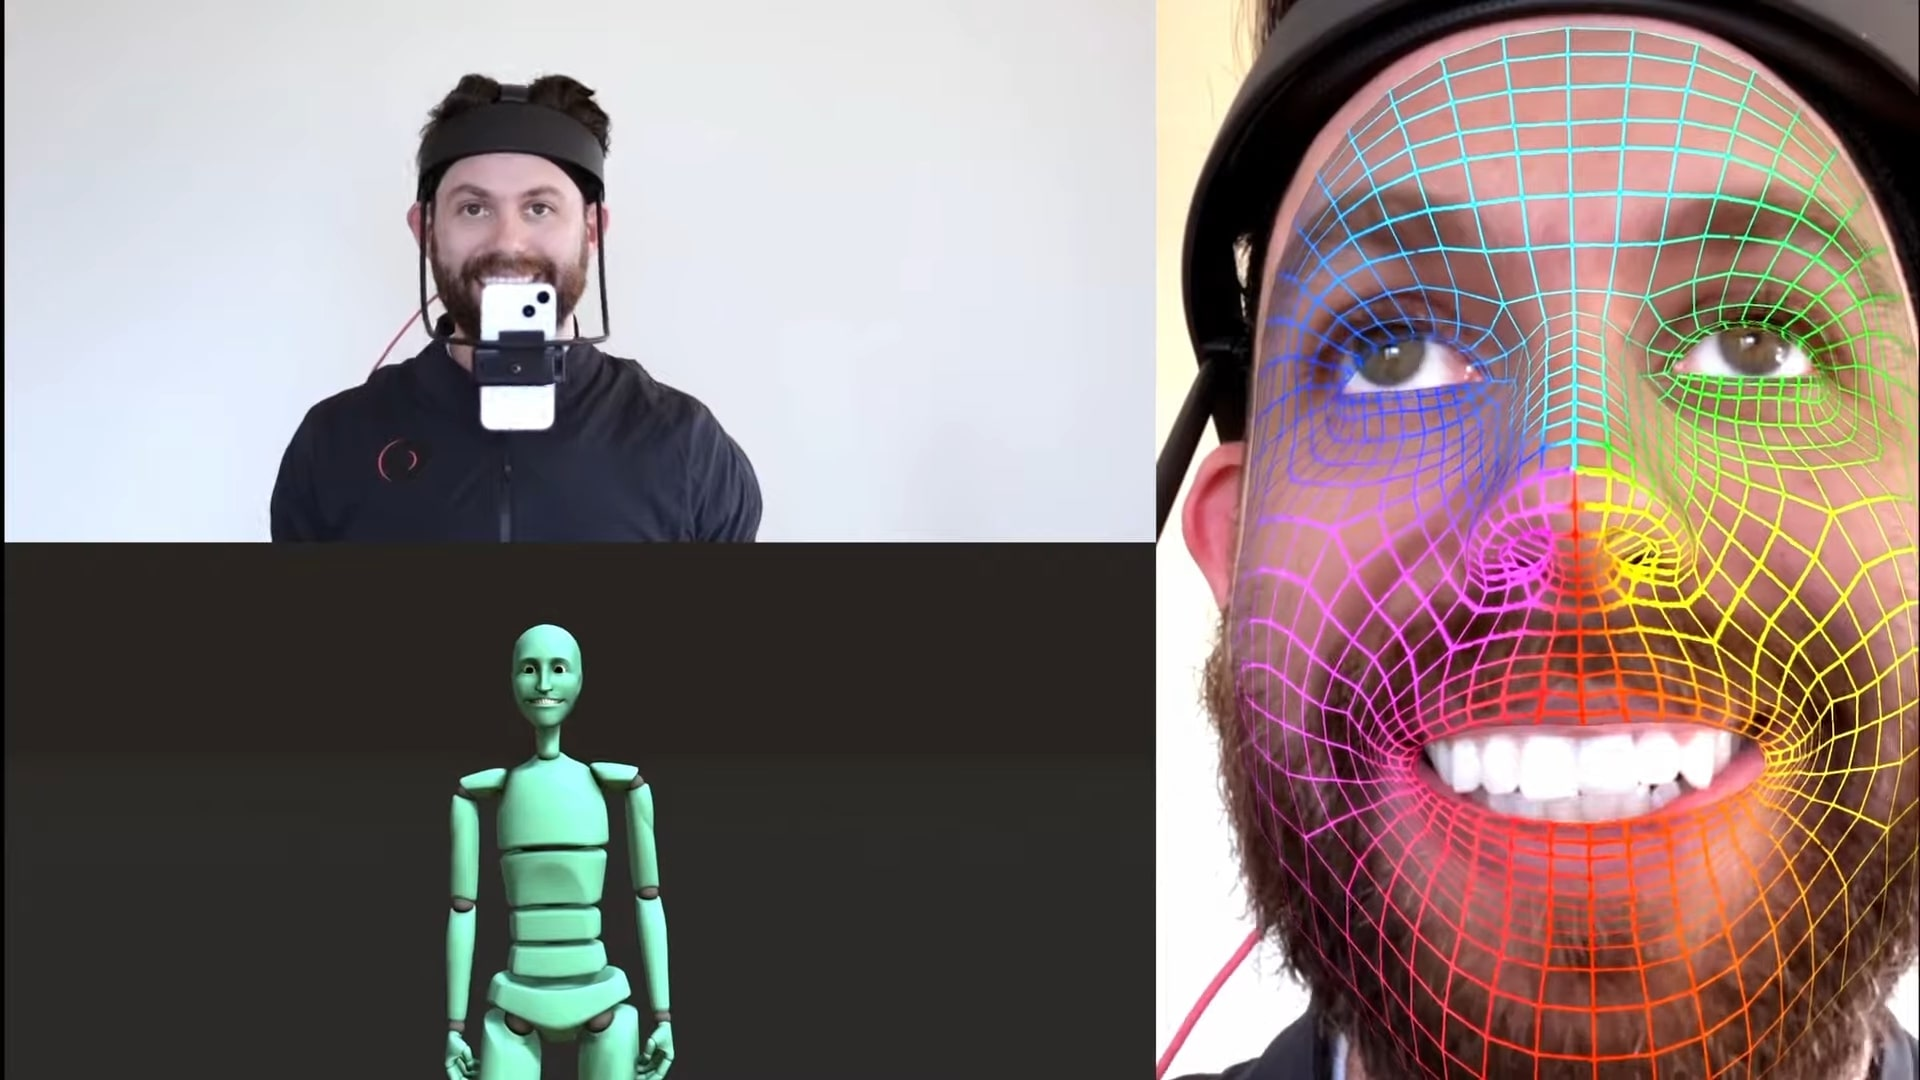
\includegraphics[width=0.8\textwidth]{chapters/facial_expressions/images/motion_capture.png}
    \caption{Performance-based facial animation using motion capture technology, which captures the real-time movements of an actor’s face.}
    \label{fig:motion_capture}
\end{figure}

\section{Action Unit Analysis}
\label{ch:facial_expressions:action_unit_analysis}

Our method for facial expression synthesis is based on the creation of blendshapes from action units (AUs), which are the fundamental building blocks of facial expressions as defined by the Facial Action Coding System (FACS). This section outlines the steps involved in our method, from the analysis of action units to the creation of blendshapes and the generation of motion curves.

The first step in our method is the analysis of action units (AUs). AUs represent the activation of specific facial muscles and are the basic components of facial expressions. Each AU corresponds to a particular movement, such as raising the eyebrows or pursing the lips, and can be combined with other AUs to create complex expressions.

To analyze AUs, we used a combination of manual observation and automatic detection tools. Manual observation involved studying facial expressions in video recordings of sign language, paying close attention to the movements of individual facial features. We also used automatic detection tools, such as FaceTorch, to identify AUs in still images. While these tools provided a useful starting point, they often required manual adjustments to ensure accuracy, particularly for subtle or complex expressions.

In cases where automatic detection fell short, particularly for expressions that involve multiple, subtle AUs, we manually annotated the facial expressions using FACS-based coding. This process involved detailed analysis of the facial expressions in our reference corpus (the 40 brèves corpus), breaking down each expression into its constituent AUs. This approach allowed us to ensure that our blendshapes accurately reflected the intended expressions, capturing both the emotional and grammatical nuances required for sign language synthesis.

\section{Blendshape Creation}
\label{ch:facial_expressions:blendshape_creation}

Once the AUs were identified, we created blendshapes that correspond to each AU. Blendshapes are essentially different versions of a 3D face model, each representing a specific facial expression. By blending these shapes together, we can create a wide range of facial expressions.

We used the FACSHuman plugin for MakeHuman to create these blendshapes. FACSHuman allows for precise control over the movement of facial features, making it possible to model each AU accurately. For each blendshape, we adjusted the position of vertices in the 3D model to match the desired facial movement. This process involved iterating between manual adjustments and automated tools to ensure that the blendshapes accurately captured the intended expressions.

The creation of blendshapes also involved ensuring that they could be seamlessly combined to create complex expressions. For example, the blendshape for AU4 (Brow Lowerer) was designed to work in conjunction with AU6 (Cheek Raiser) and AU12 (Lip Corner Puller) to create expressions of anger or determination. This required careful coordination of the vertex movements across different blendshapes to avoid unnatural deformations or artifacts in the final animation.

\subsection{Motion Curves for Blendshapes}
\label{ch:facial_expressions:motion_curves_for_blendshapes}

After creating the blendshapes, we generated motion curves to control how these shapes are animated over time. Motion curves define the changes in the blendshape's influence over the course of an animation, allowing for smooth transitions between different facial expressions.

We extended our intermediate block generator to include motion curves for facial morphs. This involved creating additional curves that specify the timing and intensity of facial movements based on the AZee production rules. By controlling the acceleration and deceleration of these movements, we were able to create more naturalistic animations that reflect the dynamic nature of facial expressions.

For example, in the expression "big-threatening," the motion curves were designed to gradually increase the influence of the blendshapes corresponding to AU10 (Upper Lip Raiser) and AU25 (Lips Part) while simultaneously decreasing the influence of AU4 (Brow Lowerer) as the expression transitions from a neutral state to one of aggression. This careful modulation of the blendshape influences over time resulted in an expression that not only looked realistic but also conveyed the intended emotional and grammatical cues effectively.

\section{Results and Implementation}
\label{ch:facial_expressions:results}

Our method was evaluated through the synthesis of facial expressions on a set of signing avatars. We tested the avatars' ability to perform a wide range of AUs and combined them to create the expressions defined by the AZee production rules. The results were assessed based on the realism of the animations, the accuracy of the expressions, and the ability to apply them consistently across different avatars.

The synthesized facial expressions were tested with native sign language users to assess their effectiveness in conveying both emotional and grammatical information. Preliminary feedback indicated that the expressions were generally well-received, with users noting improvements in the realism and expressiveness of the avatars compared to previous models. However, some limitations were identified, particularly in the modeling of certain complex expressions, which we discuss in the following section.

One notable success was the synthesis of expressions related to questions and emphasis, which are heavily reliant on precise eyebrow and eyelid movements. The blendshapes and motion curves for these expressions were particularly effective in conveying the necessary non-manual signals, enhancing the overall comprehension of the signed messages. However, expressions that involved subtle mouth movements, such as "it-is-a-shame" or "something-sticks-out," were more challenging to model accurately, highlighting areas for further refinement.

\section{Evaluation}
\label{ch:facial_expressions:evaluation}

todo

\section{Conclusion}
\label{ch:facial_expressions:conclusion}

todo

\end{document}